\section{Das MapReduce-Framework}
MapReduce wurde 2004 von zwei Mitarbeitern von Google vorgestellt \cite{dean2008mapreduce}. Es ist ein Framework
für die Entwicklung von massiver, paralleler Datenverarbeitung sehr großen Datenmengen auf Clustern.

Der Programmierer
kann sich dabei komplett auf die Verarbeitung der Daten konzentrieren. Das Framework kümmert sich um die parallele
Ausführung der Arbeit, ohne dass der Programmierer der Anwendung wissen muss, welche Daten konkret wo verteilt vorliegen
und verarbeitet werden. 
Im Zusammenarbeit mit speziellen Filesystemen 
für große Cluster-Systeme, die zum Beispiel automatisch redundante Kopien auf mehreren Maschinen anlegen, ermöglicht
eine mit MapReduce programmierte Anwendung zudem eine hohe Toleranz gegenüber dem Ausfall von einzelnen Maschinen.

\subsection{Arbeitsweise von MapReduce}
Auf der obersten Abstraktionsebene besteht das MapReduce-Framework nur aus zwei spezifizierten Funktionen: \textit{map} und \textit{reduce}.
Beide Funktionen müssen vom Anwender des MapReduce-Frameworks implementiert werden.
\textit{Map} nimmt eine, möglicherweise ungeordnete, Liste von Daten entgegen, die Schlüssel-Wert-Paare (key/value) enthält. Die Funktion 
verarbeitet nun diese Liste nach dem vom Programmierer implementierten Funktion und liefert als Ergebnis wiederum eine
Liste von Schlüssel-Wert-Paaren. Die konkrete Logik der \textit{Map}-Funktion ist vom Anwendungsfall abhängig, bildet aber in der Regel
ungeordneten Daten in eine Liste ab, die die für den Anwendungsfall interessanten Daten enthält. 


%Beispiel?
%Ein gern genommenes Beispiel
%ist das Zählen von Wörtern in tausenden von Dokumenten. Die Liste für die Eingabe in die \textit{map}-Funktion enthält für jeden Schlüssel
%als Wert ein ganzes Dokument. Diese Dokumente werden durchsucht und gleichzeitig eine neue, deutlich größere Liste mit Schlüssel-Wert-Paaren erstellt, 
%die für jedes einzelne Wort den String selbst als Schlüssel speichert, und als Wert eine 1 angibt. Somit ist jedes Wort in dieser Liste repräsentiert.
%Diese neue Liste enthält sehr viele gleiche Schlüssel, wobei alle den Wert 1 tragen.

Das Ergebnis von der \textit{Map}-Funktion ist aber nur ein Zwischen-Ergebnis und wird direkt als Eingabe für die \textit{Reduce}-Funktion verwendet,
die am Ende das tatsächliche Ergebnis der Verarbeitung ausgibt. Die \textit{Reduce}-Funktion hat in der Regel die Aufgabe, das Ergebnis der \textit{Map}-Funktion
zusammenzufassen.  

%Bezogen auf das Beispiel mit der Zählung von Wörtern bekommt die \textit{reduce}-Funktion nun eine (sehr lange) Liste von allen Wortvorkommnissen.
%Die Funktion sortiert  nun diese Liste und erzeugt eine neue Liste, die alle Schlüssel-Werte enthält, aber nur ein einziges mal in der Liste. Mehrfache Einträge
%in der ursprünglichen Liste mit gleichen Schlüsselwerten werden also zu einem Eintrag zusammengefasst, wobei die Werte der einzelne, mehrfachen Einträge
%aufaddiert werden. Das Ergebnis ist eine Liste mit jedem Wort, das in den Dokumenten vorkommt, als einmaliger Schlüssel und als Wert die jeweilige Häufigkeit.

Neben den beiden Funktionen \textit{map} und \textit{reduce} liefert das MapReuce-Framework auch eine Laufzeitumgebung mit, in der jene beiden Funktionen eingebettet sind.
Die Laufzeitumgebung kümmert sich dabei um die Verteilung der Arbeit auf dem Cluster. 
Dafür werden erstens die implementierten \textit{Map-} und \textit{Reduce}-Funktionen
kopiert und auf die einzelnen Maschinen im Cluster verteilt. Zweitens werden die Eingabedaten zerteilt und die einzelnen Daten-Stücke auf die Maschinen verteilt. 

Die konkrete Implementierung der Laufzeitumgebung hängt vom Einsatzort und Zweck ab. 
Google schlägt in seinem Paper folgendes Konstrukt vor, das in Abbildung \ref{fig:mapreduce} visualisiert wird.

\begin{figure}[H]
\centering
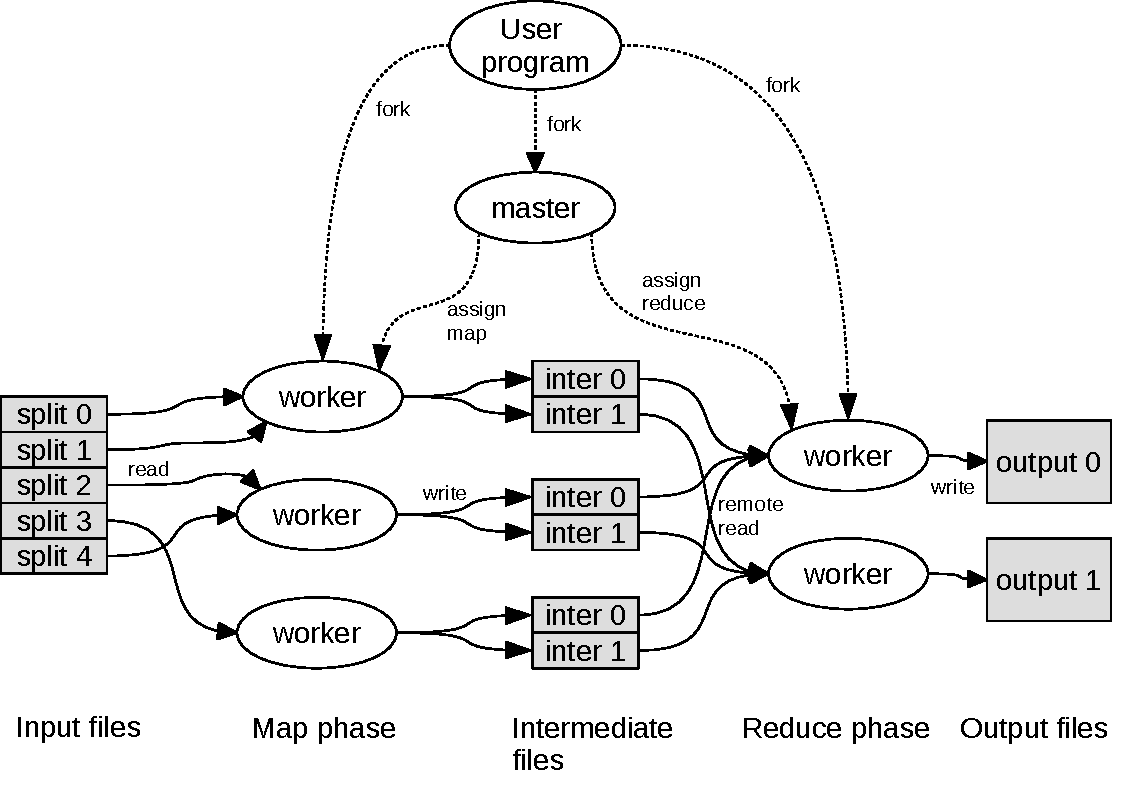
\includegraphics[width=1.0\textwidth]{images/06mapreduce.pdf}
\caption{MapReduce-Laufzeitumgebung wie von Google vorgeschlagen. \cite{miner2012mapreduce}}
\label{fig:mapreduce}
\end{figure}

Die Verarbeitung von Daten mittels MapReduce läuft dann folgendermaßen ab:

Die Eingabedateien werden in $M$ gleich große Teilstücke von üblicherweise $16 MB$ bis $64 MB$
aufgeteilt. Das vom Nutzer implementierte Programm enthält die \textit{Map}- und 
\textit{Reduce}-Funktionen. Die einzelnen Maschinen (\textit{worker}) im Cluster bekommen jeweils
eine Kopie des Programms. Dabei ist eine einzige Kopie der Master, der sich anschließend
um die Koordination der Arbeit kümmert. Mit den $M$ gleich großen Teilstücken stehen nun
auch $M $ \textit{Map}-Aufgaben bereit zur Verarbeitung. Anschließend wird auch die Anzahl der Teilstücke
der Zwischenergebnisse $R$ ermittelt. Diese Anzahl $R$ stellt dann die Menge der verfügbaren
\textit{Reduce}-Aufgaben dar.

Nach dieser Vorbereitung kann die Arbeit nun schließlich beginnen. Dafür schaut der Master nach,
welche Maschinen beziehungsweise Worker nicht beschäftigt sind und weist ihnen entweder eine \textit{Map}- oder \textit{Reduce}-Aufgabe zu. Die \textit{Map}-Worker beginnen nun
die ihnen zugewiesenen Dateien zu bearbeiten, die aus Schlüssel-Wert-Paaren bestehen und
erzeugen die Zwischen-Dateien. Die Zwischen-Ergebnisse sind ebenfalls nach Schlüssel-Wert-Paaren
strukturiert. Die Zwischen-Ergebnisse werde dabei in $R$ Teil-Bereiche eingeordnet, abhängig
von ihrem Schlüssel-Wert.

Sobald ein oder mehrere \textit{Map}-Aufgaben erledigt sind, teilt der Master ein oder mehreren 
\textit{Reduce}-Workern, die gerade nichts zu tun haben, mit, dass sie mit der Verarbeitung beginnen können. Der Master teilt ihnen dabei auch mit, wo die entsprechenden Zwischenergebnisse liegen,
die sie verarbeiten sollen. Die \textit{Reduce}-Workers verarbeiten nun diese Dateien und erzeugen
mit ihrer Ausgabe einen Teil des End-Ergebnisses.


\subsection{Beispiel}
Als Beispiel dient die Analyse einer großen Datenmenge von Musiksongs mit Hilfe von MapReduce. Die Daten liegen als
Schlüssel-Wert-Paare vor. Jeder Song hat dabei einen eigenen Schlüssel, die Song-ID, sowie eine Reihe von Song-Informationen als Wert.
Die Song-Informationen beinhalten Daten wie Name des Songs, der Künstler, Beats per minute, aktueller Rank in den Charts etc.

Wir wollen nun in diesem sehr großen Datensatz an Songs herausfinden, welcher Künstler wie viele Songs geschrieben hat. Wir gehen in diesem Beispiel davon aus, dass wir eine Kenntnis davon haben, welche Künstler in  dem Datensatz vorkommen.
Im ersten Schritt müssen wir die \textit{Map}-Funktion beschreiben. Sie bekommt als Eingabe eine Reihe von Songs mit der Song-ID
als Schlüssel und ihren Eigenschaften als Werte. Diese Songs werden nun direkt auf ein Zwischenergebnis gemappt, indem der
Künstler-Name als Schlüssel und die Zahl $1$ als Wert geschrieben werden. Dies führt zu einem (großen) Zwischenergebnis,
bei dem die Anzahl der Vorkommnisse eines Künstlernames die Anzahl seiner Songs wiedergibt. Das muss aber
natürlich noch als Endergebnis zusammen gefasst werden, was dann die \textit{Reduce}-Funktion übernimmt. 

Die \textit{Reduce}-Funktion bekommt vom Master einen Werte-Bereich aus dem Zwischenergebnis zugewiesen, die sie auf
ein Endergbnis reduzieren soll. Sie holt sich dann anschließend diesen Wertebereich des Zwischenergebnisses von den verteilten
\textit{Map}-Maschinen. Sie fasst nun alle gleichen Schlüssel zu einem einzigen Schlüssel zusammen und addiert 
ihren Wert jeweils auf. Da der Wert immer $1$ ist, steht am Schluss neben dem Künstler-Name die Anzahl seiner geschriebenen
Songs. Dieses Ergebnis schreibt die  \textit{Reduce}-Funktion nun als Ergebnis raus. Die Abbildung \ref{fig:mapreduceExample} zeigt 
das Beispiel anschaulich.

\begin{figure}[H]
\centering
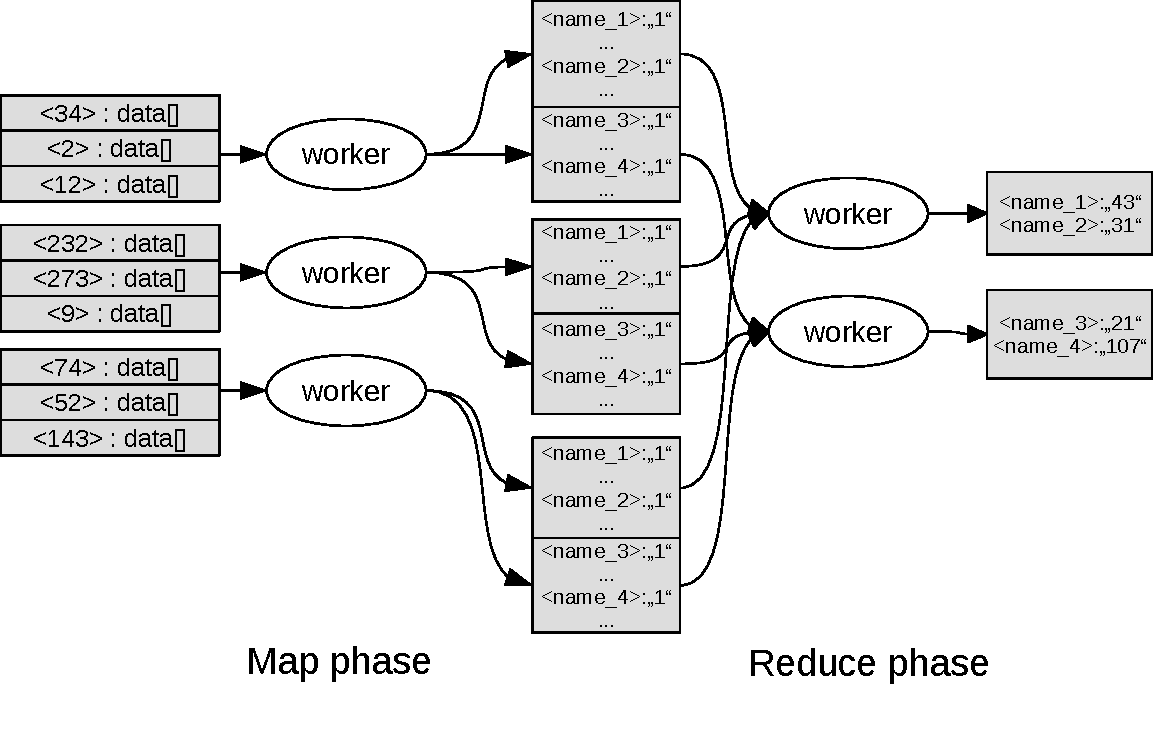
\includegraphics[width=1.0\textwidth]{images/06mapreduceExample.pdf}
\caption{Ermittlung der Anzahl der Songs für jeden Künstler mittels MapReduce.}
\label{fig:mapreduceExample}
\end{figure}

%\subsection{Implementierung von MapReduce-Funktionen}

Dieser Abschnitt beschreibt die Implementierung von Map-Reduce-Funktionen, die auf den Daten
des Million-Song-Datensatzes arbeiten. Vorausgesetzt wird, dass der Million-Song-Datensatz als
CSV-Datei bereit in das HDFS-Dateisystem importiert ist. Die hier vorgestellten MapReduce-Funktionen
arbeiten ausschließlich mit Daten auf dem HDFS-Dateisystem, abgesehen von den Zwischenergebnissen,
die auf dem lokalen Dateisystem des jeweiligen Knotens abgelegt werden.


